\begin{definition}[Notación de Funciones]
    $\boldsymbol{F}:A\subseteq \mathbb{R}^n \rightarrow B \subseteq \mathbb{R}^m$
    es una función que a cada vector de $A$ le asigna un único vector en el conjunto $B$.
    \begin{example}
        La función $\boldsymbol{T}:\mathbb{R}^2 \rightarrow \mathbb{R}^3 / \boldsymbol{T}(x,y) = (x+y,x-y,xy)$
        es un campo vectorial que asigna a cada vector de $\mathbb{R}^2$ un único vector de $\mathbb{R}^3$.
        \begin{equation*}
            \Rightarrow \boldsymbol{T}(1,1)=(2,0,1)
        \end{equation*}
        \label{ej:campoVectorial}
    \end{example}
\end{definition}
\begin{definition}[Dominio de una función]
    Si se tiene una función $\boldsymbol{F}:A\subseteq \mathbb{R}^n \rightarrow B \subseteq \mathbb{R}^m$
    se llama, análogamente a una función en $\mathbb{R}$, dominio a el conjunto de la salida de la función, $A$.
\end{definition}
\begin{definition}[Imágen de una función]
    Se llama imágen de una función \newline$\boldsymbol{F}:A\subseteq \mathbb{R}^n \rightarrow B \subseteq \mathbb{R}^m$ al conjunto:
    \begin{equation*}
        \text{Img}(\boldsymbol{F})={\boldsymbol{Y}\in\mathbb{R}^m: \boldsymbol{F}(\boldsymbol{X})=\boldsymbol{Y}, \boldsymbol{X} \in A}
    \end{equation*}
    Esto es análogo a las funciones en $\mathbb{R}$.
\end{definition}
\begin{definition}[Campo Escalar]
    Un campo escalar es una función $f:A\subseteq \mathbb{R}^n \rightarrow B \subseteq \mathbb{R}$, tal que asigna
    a un vector (o escalar) perteneciente a $A\subseteq \mathbb{R}^n$ un escalar real.
    Un campo escalar se nota con una letra minúscula de imprenta.
    \begin{example}
        La función $d:\mathbb{R}^3 \rightarrow \mathbb{R} / d(x,y,z) = \sqrt{x^2+y^2+z^2}$
        es un campo escalar que asigna a cada vector de $\mathbb{R}^3$ un escalar. 
        En particular, si se piensa el vector argumento como un punto en el espacio, $d$ devuelve su distancia euclidea al orígen.
        \begin{equation*}
            \Rightarrow d(1,2,3)=\sqrt{1^2+2^2+3^2}=\sqrt{14}
        \end{equation*}
        \label{ej:campoEscalar}
    \end{example}
\end{definition}
\begin{definition}[Campo Vectorial]
    Se llama campo vectorial a una función $\boldsymbol{F}:A\subseteq \mathbb{R}^n \rightarrow B \subseteq \mathbb{R}^m$
    donde $n\geq2$ y $m\geq2$. Es decir, donde se asigna un vector de un espacio real de dimensión al menos 2 y se devuelve otro
    en un espacio (igual o distinto) de, también, dimensión al menos 2. 
    A un campo vectorial se lo llama con una letra mayúscula de imprenta.
    
    La función del ejemplo (\ref{ej:campoVectorial}) es un campo vectorial.

    Sea $\boldsymbol{F}(x_0,x_1,...,x_n)=(y_0,y_1,...,y_m)$ un campo vectorial, el vector que devuelve
    se puede pensar como la evaluación de $m$ campos escalares en $(x_0,x_1,...,x_n)=\boldsymbol{X}$. 
    Es decir:
    \begin{equation*}
        \boldsymbol{F}(\boldsymbol{X})=(f_0(\boldsymbol{X}),f_1(\boldsymbol{X}),...,f_m(\boldsymbol{X}))
    \end{equation*}
    Donde $f_0,f_1,...,f_m$ se llaman las \textbf{componentes de} $\boldsymbol{F}$.

    Volviendo al ejemplo (\ref{ej:campoVectorial}), las componentes de $T$ son: 
    \begin{equation*}
        f_1(x,y)=x+y\qquad f_2(x,y)=x-y\qquad f_3(x,y)=x+y
    \end{equation*}
\end{definition}
\begin{definition}[Parametrización]
    Se llaman parametrizaciones a las funciones de la forma $\boldsymbol{\sigma}:A\subseteq\mathbb{R}\rightarrow B\subseteq\mathbb{R}^n$
    donde $n\geq2$. Es decir, a las funciones que asignan a cada escalar real en el conjunto $A$
    un vector perteneciente a $\mathbb{R}^n$.
    Una parametrización se los suele notar con una letra griega.

    Si se piensa a los vectores de salida como puntos en el plano ($\mathbb{R}^2$) o en el espacio ($\mathbb{R}^3$),
    la imágen de una parametrización es un conjunto de puntos que conforman una curva.

    \begin{example}[Parametrización de la circunferencia]
        Para parametrizar una circunferencia, primero pensemos en el circulo unitario.
        En el circulo unitario, la abcisa (coordenada x) de cualquier punto es el coseno del ángulo que forma el eje horizontal con el segmento de radio
        que une el origen con tal punto. Asimismo, el seno del ángulo representa la ordenada (coordenada y).
        \begin{figure}[H] 
            \centering
            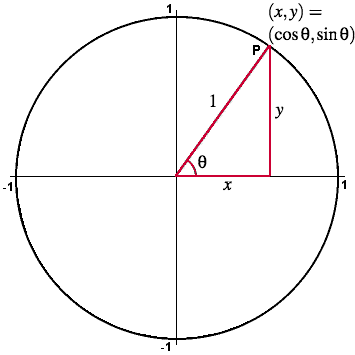
\includegraphics[width=0.5\textwidth]{../figs/unitCircle1.png} % Cambia esta ruta por la ubicación de tu imagen
            \caption{Coordenadas de los puntos sobre una circunferencia unitaria.}
            \label{fig:unitCircle1} % Etiqueta para hacer referencia a la imagen
        \end{figure}
        Por lo tanto, se propone una parametrización de la circunferencia unitaria de la forma:
        \begin{equation*}
            \boldsymbol{\sigma}:[0,2\pi)\rightarrow\mathbb{R}^2/ \\ \boldsymbol{\sigma}(t)=(\cos{t},\sin{t})
        \end{equation*}
        Así, si se graficase $\text{Img}(\boldsymbol{\sigma})$ como puntos en el plano se obtendría toda la circunferencia unitaria.
        Vale aclarar que se tomó el dominio como cerrado en $0$ y abierto en $2\pi$, para que, puesto que ambos valores de 
        entrada corresponden al mismo punto de salida, la parametrización no tenga "puntos repetidos", es decir, que sea inyectiva 
        (análogo a la inyectividad de funciones de $\mathbb{R}$ a $\mathbb{R}$).

        Para contemplar circunferencias de radio distinto de 1, vale con multiplicar el radio a cada componente de la parametrización.
        Además, para parametrizar aquellas que no estén centradas en el orígen, se desplaza cada punto de salida de la
        parametrización por $(x_0,y_0)$, el centro de la nueva circunferencia.
        Por lo tanto, la parametrización de una circunferencia de radio $r\in\mathbb{R}^+$ centrada en $(x_0,y_0)$ es:
        \begin{equation*}
            \boldsymbol{\sigma}:[0,2\pi)\rightarrow\mathbb{R}^2/ \\ \boldsymbol{\sigma}(t)=(r\cdot\cos{t}+x_0,r\cdot\sin{t}+y_0)
        \end{equation*} 
    \end{example}
\end{definition}